\section{Inner circle method}
\label{sec:proof_inner_circle}
\begin{figure}[htbp]
    \centering
    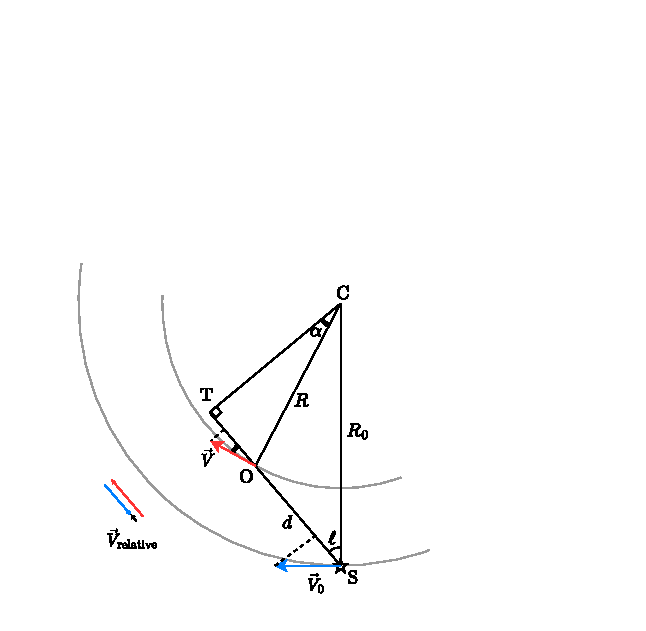
\includegraphics[width=0.5\textwidth]{figures/inner_circle_method.pdf}
    \caption{Schematic of the inner circle method}
    \label{fig:inner_circle_method}
\end{figure}
%
The velocity of the observed galactic object O given the relative velocity $V_\textrm{relative}$ projected on the line of sight axis ST between the observer S and the object is given by
\begin{equation}
    V = \frac{R}{R_0} \left( \frac{V_\textrm{relative}}{\sin(\ell)} + V_0 \right)
\end{equation}
\begin{proof}
    Using trigonometry, the distance TC can be written as
    \begin{equation}
       \textrm{TC} = R_0 \sin\ell = R \cos\alpha
       \label{eq:proof1}
    \end{equation}
    % and
    % \begin{equation}
    %     \textrm{TO} = R_0 \cos\ell - d = R \sin\alpha
    %    \label{eq:proof2}
    % \end{equation}
    The projected relative velocity is given by
    \begin{equation}
        V_\textrm{relative} = V \cos\alpha - V_0 \sin\ell
       \label{eq:proof3}
    \end{equation}
    From \autoref{eq:proof1}, it is clear that $\cos\alpha = \frac{R_0}{R} \sin\ell$. Substituting in \autoref{eq:proof3}, we get
    \begin{equation}
        V_\textrm{relative} = \left( \frac{R_0}{R} V - V_0 \right) \sin\ell
    \end{equation}
    By rearanging this equation, the final result can be found
    \begin{equation}
        V = \frac{R}{R_0} \left( \frac{V_\textrm{relative}}{\sin(\ell)} + V_0 \right)
    \end{equation}
\end{proof}
